% app_network_results.tex -- the network results of the detach and attach sections on the earlier plant,
% moved here 11 Oct when the planner-against-network question became Appendix F. Text as drafted 4 Oct.

\subsection{Detach and attach with the network on the earlier plant}
\label{sec:app_network_results}

\paragraph{OCP resize against network hand-off.} Table~\ref{tab:detach_ab} compares the two detach
methods of Section~\ref{sec:reconfig} on the same flight: four UAVs flying a circle, one released
mid-way. The flights used an early payload (0.4\,kg, 0.5\,m cables, circle at 0.6\,m/s). With the OCP
resize the payload settled level and the survivors kept tracking their references. With the network
hand-off the payload settled tilted by 26--48$^\circ$, and the survivors were 0.06--0.91\,m off their
references while the network redistributed the load. Two fixes were needed for the network sequence
to hand back to the planner at all: the feedforward soft-start must not restart on an airborne
hand-back, and the new solver must be primed before it flies. Without them the payload dropped to
0.07\,m above the floor after the detach; with them it stayed above 0.46\,m.

\begin{table}[h]
\centering
\caption{Detach from four UAVs to three during a circle, Gazebo, early payload (0.4\,kg).}
\label{tab:detach_ab}
\begin{tabular}{lcc}
\toprule
 & OCP resize & Network hand-off \\
\midrule
settled payload tilt & about 1$^\circ$ & 26--48$^\circ$ \\
survivor tracking error & about 1\,mm & 60--910\,mm \\
\bottomrule
\end{tabular}
\end{table}

On the 0.86\,kg ring the gap widened. In the software-in-the-loop bench the network aborted the
flight at 53--61$^\circ$ of payload tilt after a detach, both in hover and in the circle, while the
OCP resize held the survivors level to within 0.5--2$^\circ$.

The first attach demonstration (Figure~\ref{fig:attach}) used a 0.6\,kg ring. Three UAVs at 3, 12 and
9 o'clock flew a circle at 0.2\,m/s; ATTACH held the target, and a fourth UAV welded at 6 o'clock and
was handed out by the dissipative network.

\begin{figure}[h]
\centering
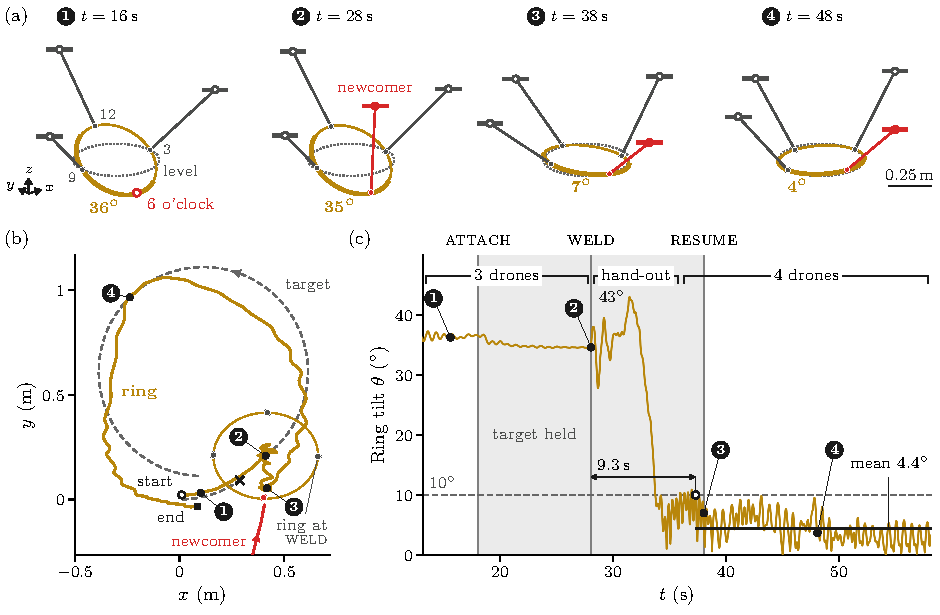
\includegraphics[width=\textwidth]{Images/attach_storyboard.pdf}
\caption[Attach during a circle]{Attach during a circle in Gazebo (0.6\,kg ring of radius 0.25\,m on 0.5\,m rods). (a) The
fleet at the four numbered instants, rebuilt from the logged poses in one orthographic view: carriers
grey, newcomer red; thick: near half of the ring; dotted: the ring if it were level; bar: 0.25\,m.
(b) Plan view of the ring centre (gold; circle: start, square: end), the payload target (dashed; x:
held from ATTACH) and the newcomer's approach (red), with the ring and its rim anchors at the weld.
(c) Ring tilt; grey band: target held; dashed: 10$^\circ$. Three UAVs at 3, 12 and 9 o'clock start
the circle with the ring tilted by 34--37$^\circ$. ATTACH holds the target and the newcomer welds to
the empty 6 o'clock rim. During the 8\,s hand-out the tilt first rises to 43$^\circ$; from 9.3\,s
after the weld it stays under 10$^\circ$ (mean 4.4$^\circ$, peak 9.96$^\circ$), and the four UAVs fly
the rest of the circle, 0.20\,m RMS from the target against 0.02\,m with three.}
\label{fig:attach}
\end{figure}

The sequence completed in every repeat, but it exposed two limits. First, three UAVs on a ring hang it
tilted when their attachment points leave the centre of mass on the edge of their support triangle:
at 3/12/9 o'clock the ring hung 27--37$^\circ$ before the weld. The fourth UAV is what levels it.
Second, the layout trades a level hover against a level circle (Table~\ref{tab:attach_layout}). At
3/12/9 o'clock plus 6 the hover is tilted and the four-UAV circle is level. At 4/12/8 o'clock plus 6
the hover is level, but the UAV at 12 o'clock carries about 40\,\% of the load against 20\,\% for the
others, and the four-UAV circle rolled by 20--37$^\circ$. A tracker without an integrator sags in
proportion to its force error, so the most heavily loaded UAV sags most, and a common-mode trim cannot
correct a differential sag.

\begin{table}[h]
\centering
\caption{Network attach on the 0.6\,kg ring by layout (Gazebo).}
\label{tab:attach_layout}
\small
\begin{tabularx}{\textwidth}{>{\raggedright\arraybackslash}Xccc}
\toprule
Layout & Three-UAV hover tilt & Weld transient & Four-UAV circle tilt \\
\midrule
3/12/9 o'clock, newcomer at 6 & 33$^\circ$ & 47$^\circ$ peak, 12\,s to settle & 3.7$^\circ$ mean \\
4/12/8 o'clock, newcomer at 6 & 2.0$^\circ$ & 10$^\circ$ mean over 4\,s & 20--37$^\circ$ roll \\
\bottomrule
\end{tabularx}
\end{table}

On the 0.86\,kg ring the network attach capsized the payload within about 8\,s of every weld in the
software-in-the-loop bench, while the OCP resize held the same weld at a peak of about 10$^\circ$, in
hover and in the middle of a circle. The attach was therefore moved to the OCP resize.
